\documentclass[11pt,a4paper]{report}
\usepackage[margin=25mm]{geometry}
\usepackage{amsmath,amssymb,booktabs,longtable,array,graphicx,xcolor,listings}
\usepackage{tikz}
\usetikzlibrary{arrows.meta,positioning}
\usepackage[hidelinks,hypertexnames=false]{hyperref}
\usepackage{microtype}
\usepackage{fancyhdr}
\pagestyle{fancy}\fancyhf{}\fancyhead[L]{Updated quantum fidelity attention}\fancyfoot[C]{\thepage}
\setlength{\headheight}{15pt}
\setlength{\emergencystretch}{3em}
\lstset{basicstyle=\ttfamily\scriptsize,breaklines=true,columns=fullflexible,keepspaces=true,showstringspaces=false,frame=single,keywordstyle=\color{blue!60!black},commentstyle=\color{green!40!black},stringstyle=\color{red!50!black}}
\newcommand{\ket}[1]{\lvert #1\rangle}
\newcommand{\bra}[1]{\langle #1\rvert}
\newcommand{\code}[1]{\texttt{\detokenize{#1}}}
\title{Detailed Implementation and Evaluation Report\\[8mm]\large Native-Resolution Pneumonia Classification with a Frozen Image Encoder and Four-Qubit Quantum Fidelity Attention}
\author{Updated project documentation\\Source, checkpoints, and verification evidence retained in \texttt{UPDATED}}
\date{2 October 2026}
\begin{document}
\maketitle
\begin{abstract}
This report documents the completed version of the project that exceeds 90\% test accuracy while retaining quantum-circuit attention. Official native 224-pixel PneumoniaMNIST images are processed by a frozen ImageNet-pretrained ResNet-18. Four spatial feature tokens are projected into a small transformer whose query--key similarities are four-qubit state fidelities. The entangled feature map uses angle encoding, a CNOT chain, and a second data-encoding stage. A product-state circuit and a parameter-matched classical dot-attention model provide controls. Training uses AdamW, training-only feature normalization and flip views, feature MixUp, exponential moving average parameters, and validation-based checkpoint selection and temperature calibration.

Across five seeds, entangled quantum attention achieves 91.60\% $\pm$ 0.58\% single-model accuracy and 91.67\% ensemble accuracy (572 of 624 test images). Product quantum attention achieves 91.19\% ensemble accuracy; the matched classical dot ensemble achieves 92.15\%. Independent PennyLane compute--uncompute inference reproduces every quantum classifier's decisions on the complete test split. These results establish a working, reproducible hybrid classifier, but do not demonstrate quantum superiority, quantum speedup, algorithmic novelty, or clinical readiness. The official test cohort had been examined in earlier experiments, so this study is exploratory. Native resolution and external pretraining change the comparison regime relative to the earlier 88.94\% result.
\end{abstract}
\tableofcontents
\listoffigures
\listoftables

\chapter{Purpose, scope, and the meaning of the result}
\section{The problem being solved}
The task is binary classification of chest radiograph images in PneumoniaMNIST: label 0 denotes normal and label 1 denotes pneumonia. The engineering objective was to improve the earlier project's accuracy beyond 90\%, while keeping an actual quantum algorithm in the inference path. The resulting architecture is a hybrid model: classical image processing produces features, a quantum feature map supplies attention similarities, and classical layers aggregate these similarities into a prediction.

An image does not enter a quantum device directly. The encoder first extracts useful visual structure. A learned projection then compresses each token into four query or key coordinates. Those coordinates determine quantum rotation angles. The overlap between two encoded states answers the attention question: how similar is this token's query to another token's key?

\section{What has actually been achieved}
All ten quantum classifiers---five entangled and five product-state models---exceed 90\% on the 624-image official test split. The main entangled ensemble correctly classifies 572 images and misclassifies 52. All fifteen neural models and a classical linear control are retained. Their complete prediction arrays, training histories, best checkpoints, resumable checkpoints, and verification records accompany this report.

The current quantum algorithm is \emph{compute--uncompute fidelity estimation}. Training uses a differentiable statevector simulator that evaluates the same gate circuit. Independent inference executes the corresponding circuit in PennyLane. Neither execution uses a physical quantum processing unit (QPU); there are no sampled measurement shots in this accuracy result.

\section{What this result cannot establish}
The new entangled ensemble improves the older 88.9423\% reference by approximately 2.72 percentage points, equivalent to 17 more correct predictions on this cohort. However, the new experiment also adds external ImageNet pretraining and higher-resolution source images. Therefore this improvement cannot be attributed exclusively to quantum attention. The matched classical ensemble is more accurate than the quantum ensemble. A successful course project is supported; a claim that the quantum method is the best classifier or a newly invented publishable algorithm is not supported by these results.

The test cohort was inspected during earlier research. Validation-only selection within the new experiment prevents direct test-based checkpoint selection, but does not turn this repeatedly examined cohort into an independent confirmatory test. New external data and a prospectively fixed protocol would be needed for a stronger claim.

\chapter{Data and preprocessing}
\section{Official data and split roles}
The native-resolution archive is the official MedMNIST+ PneumoniaMNIST 224-pixel dataset \cite{medmnist}. It contains the following fixed splits; the project does not rearrange, subset, or merge them.
\begin{table}[htbp]\centering
\begin{tabular}{lrrr}\toprule
Split & Images & Normal & Pneumonia\\\midrule
Training & 4,708 & 1,214 & 3,494\\
Validation & 524 & 135 & 389\\
Test & 624 & 234 & 390\\\bottomrule
\end{tabular}
\caption{Official split counts. Training supplies gradients, validation supplies selection and calibration, and test supplies evaluation.}
\end{table}
The class distributions differ: approximately 74.2\% of training and validation images are positive, compared with 62.5\% of test images. Class weighting addresses imbalance in the training objective. This difference alone does not prove why an earlier model made errors.

The native archive is 214,384,716 bytes. Its official MD5 is
\begin{quote}\small\code{d6a3c71de1b945ea11211b03746c1fe1}.\end{quote}
The smaller 28-pixel reference archive is retained for cross-resolution correspondence checks. Split labels are exactly equal between the two archives. Each native image is area-downsampled to 28 pixels and compared with the same-index reference image using centered Pearson correlation. More than 99\% of each split must exceed 0.9 correlation. The measured fractions are approximately 0.999788 for training and 1.0 for validation and test. This supports correspondence of the supplied images and their ordering; it is not a patient-identity audit.

\section{Why native resolution matters}
Upscaling a 28-pixel image to 224 pixels changes its dimensions, but cannot recover anatomical detail discarded by the original downsampling. Using the supplied native 224-pixel archive provides a different input-information regime. The earlier experiment that fed enlarged 28-pixel images into the pretrained encoder reached only 86.70\% quantum ensemble accuracy. The native experiment retains the same pretrained-head training recipe and changes the raw archive and experiment namespace. Both resolution regimes remain documented.

\section{Image transformations}
The data loader represents grayscale pixels in $[-1,1]$. Before CNN inference, they are mapped back to $[0,1]$ by $(x+1)/2$. Grayscale is repeated across three channels to satisfy the pretrained network's RGB input interface; repeating a channel introduces no color information.

The official \code{IMAGENET1K_V1} weight transform resizes the shorter side to 256 pixels and center-crops to $224\times224$, followed by channel normalization \cite{resnetdocs}:
\begin{equation}
x'_c=\frac{x_c-\mu_c}{\sigma_c},\quad
\boldsymbol\mu=(0.485,0.456,0.406),\quad
\boldsymbol\sigma=(0.229,0.224,0.225).
\end{equation}
Thus ``native 224'' describes the source archive, while the CNN still uses its prescribed resize/crop transformation. The report does not imply that every source pixel survives the center crop.

Two feature views are cached for every training image: the original image and a horizontal flip applied before the CNN transform. Validation and test have only the canonical view. During each training batch, the head randomly selects one of the two cached views for each example. The final native experiment does not use the older branch's random affine, brightness, or contrast augmentation.

\section{Training-only feature normalization}
The CNN yields feature arrays of shape $[V,N,4,512]$, where $V=2$ for training and $V=1$ otherwise. A mean and sample standard deviation are estimated for each of the 512 channels over training views, images, and spatial tokens:
\begin{equation}
\widehat f_{n,t,c}=\frac{f_{n,t,c}-\mu_c^{\rm train}}
{\max(\sigma_c^{\rm train},10^{-4})}.
\end{equation}
The same stored statistics transform validation and test. No validation or test feature contributes to these fitted statistics. Caching avoids repeating the frozen CNN computation every epoch and preserves exact feature provenance. Caching a split is not fitting the model on that split.

\chapter{The classical image encoder and transformer}
\section{Frozen ResNet-18 transfer learning}
ResNet-18 learns image representations through convolutions and residual connections. A residual block adds an input pathway to a learned transformation, so its output is conceptually $x+F(x)$. This enables the network to build representations without forcing every block to reconstruct its input from scratch.

The project loads public ImageNet-1K weights, removes the network's original average-pooling and classification layers, and adds adaptive average pooling to a $2\times2$ spatial grid. At 224-pixel CNN input, the final convolutional feature map has 512 channels; pooling produces four spatial tokens with 512 features each. These tokens summarize broad spatial regions rather than raw image patches.

The encoder contains 11,176,512 parameters. All are frozen, and the encoder remains in evaluation mode: neither gradients nor batch-normalization running statistics are updated by PneumoniaMNIST. The public weight SHA256 is
\begin{quote}\small
\code{f37072fd47e89c5e827621c5baffa7500819f7896bbacec160b1a16c560e07ec}.
\end{quote}
External pretraining is part of the method and must be stated whenever its results are compared with models trained without it. Hybrid transfer learning has established prior art \cite{mari}; the use of a pretrained classical encoder followed by a quantum component is not itself a new algorithm.

\section{Token projection and sequence construction}
Each normalized 512-dimensional token passes through a trainable affine projection into 32 dimensions. A trainable classification token (CLS) is prepended, and learned positional vectors distinguish the five sequence positions:
\begin{equation}
X_0=\operatorname{Dropout}\left([x_{\rm CLS};FW_P+b_P]+P\right),
\qquad X_0\in\mathbb R^{B\times5\times32}.
\end{equation}
The CLS token accumulates information from all four spatial tokens. The head's legacy configuration contains \code{image_size=28} and \code{patch_size=14}; these fields determine only four positional-token slots. The original patch embedding layer is explicitly deleted. They do not resize the images or imply that the new encoder uses 28-pixel input.

\begin{figure}[htbp]\centering
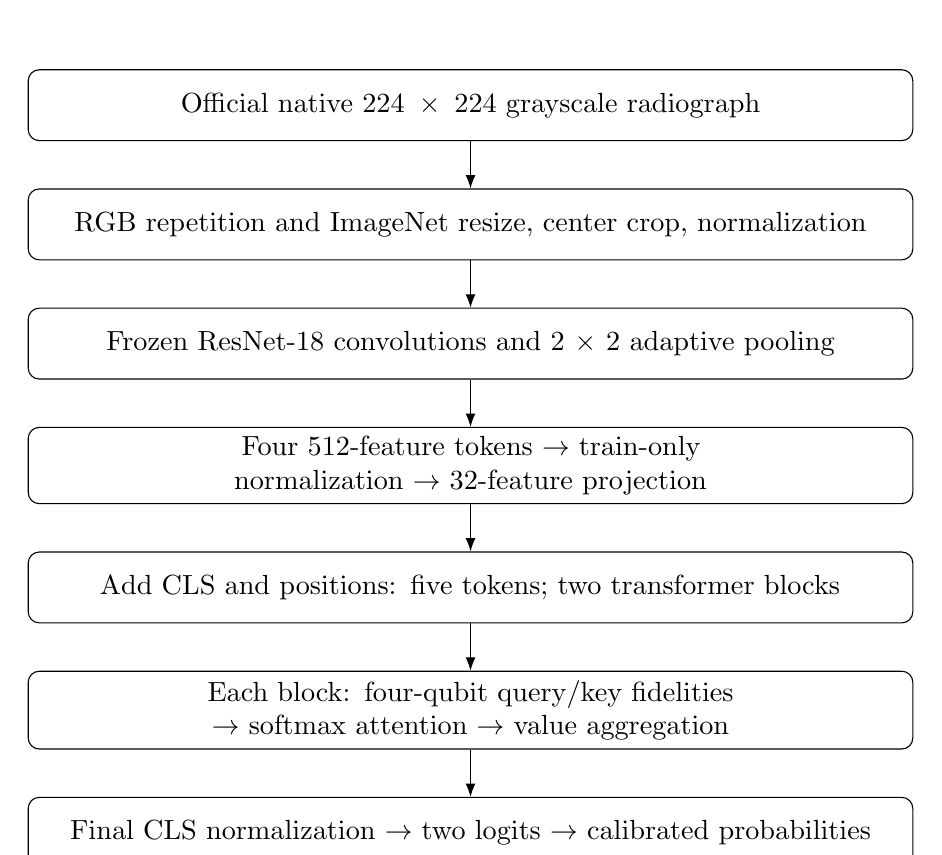
\begin{tikzpicture}[node distance=6mm,box/.style={draw,rounded corners,align=center,text width=11cm,minimum height=9mm},>=Latex]
\node[box] (a) {Official native $224\times224$ grayscale radiograph};
\node[box,below=of a] (b) {RGB repetition and ImageNet resize, center crop, normalization};
\node[box,below=of b] (c) {Frozen ResNet-18 convolutions and $2\times2$ adaptive pooling};
\node[box,below=of c] (d) {Four $512$-feature tokens $\rightarrow$ train-only normalization $\rightarrow$ $32$-feature projection};
\node[box,below=of d] (e) {Add CLS and positions: five tokens; two transformer blocks};
\node[box,below=of e] (f) {Each block: four-qubit query/key fidelities $\rightarrow$ softmax attention $\rightarrow$ value aggregation};
\node[box,below=of f] (g) {Final CLS normalization $\rightarrow$ two logits $\rightarrow$ calibrated probabilities};
\foreach \x/\y in {a/b,b/c,c/d,d/e,e/f,f/g}{\draw[->] (\x)--(\y);}
\end{tikzpicture}
\caption{The complete hybrid inference pipeline. The quantum component supplies similarities; image encoding and value processing are classical.}
\end{figure}

\section{Two pre-normalized transformer blocks}
Each block computes
\begin{align}
X'&=X+\operatorname{Attention}(\operatorname{LayerNorm}_1(X)),\\
X''&=X'+\operatorname{MLP}(\operatorname{LayerNorm}_2(X')).
\end{align}
The MLP maps $32\rightarrow64\rightarrow32$ with GELU activation and dropout. Residual additions preserve an information pathway through the block. Layer normalization stabilizes the scale of each token's features. Dropout probability is 0.1, including attention-weight dropout during training. Dropout is disabled in evaluation.

The final layer normalizes the CLS representation and applies a trainable linear map $32\rightarrow2$ to produce normal and pneumonia logits. All three neural heads have exactly 30,658 trainable parameters. The CNN parameters are not included in that trainable count.

\chapter{Quantum algorithms: gates, encoding, and fidelity}
\section{Qubits and the encoded state}
A qubit is represented as $a\ket0+b\ket1$, where $|a|^2+|b|^2=1$. Four qubits have $2^4=16$ computational-basis amplitudes. The feature map starts at $\ket{0000}$ and applies unitary gates determined by four real coordinates.

For each attention head, learned affine maps produce $q,k\in\mathbb R^4$. Each coordinate is converted into an angle using
\begin{equation}
\theta_i(z)=\frac\pi2(\tanh z_i+1).
\end{equation}
This bounds each angle between 0 and $\pi$. The mapping is differentiable, but large-magnitude coordinates can saturate the hyperbolic tangent and reduce its derivative. The model learns the query and key projection weights; it does not have an additional independent collection of variational gate parameters.

\section{Rotation gates}
The matrices used in this project are
\begin{equation}
R_Y(\theta)=\begin{pmatrix}\cos(\theta/2)&-\sin(\theta/2)\\\sin(\theta/2)&\cos(\theta/2)\end{pmatrix},
\quad
R_Z(\theta)=\begin{pmatrix}e^{-i\theta/2}&0\\0&e^{i\theta/2}\end{pmatrix}.
\end{equation}
An initial $R_Y$ creates angle-dependent amplitudes:
\begin{equation}
R_Y(\theta)\ket0=\cos(\theta/2)\ket0+\sin(\theta/2)\ket1.
\end{equation}
$R_Z$ introduces a relative complex phase. A later $R_Y$ can mix amplitudes after that phase change, allowing the final state to depend on both amplitude and phase processing.

\section{The product-state feature map}
The product control applies one $R_Y(\theta_i)$ to each wire, with no entangling gates:
\begin{equation}
\ket{\psi_{\rm product}(\boldsymbol\theta)}=
\bigotimes_{i=0}^{3}\left[\cos(\theta_i/2)\ket0+\sin(\theta_i/2)\ket1\right].
\end{equation}
Its fidelity has a direct formula:
\begin{equation}
F_{\rm product}(q,k)=\prod_{i=0}^{3}
\cos^2\left(\frac{\theta_i(q)-\theta_i(k)}2\right).
\end{equation}
This identity explains why the product kernel is efficiently classically computable. The current experiment nevertheless implements its four-qubit gates and independently checks its complete inference in PennyLane. Using a quantum-state definition is not a claim of classical computational difficulty.

For example, equal angle vectors yield fidelity 1. If three coordinates match and the remaining coordinate differs by $\pi/2$, the fidelity is $\cos^2(\pi/4)=1/2$. If one coordinate differs by $\pi$, the states are orthogonal and fidelity is 0. These examples describe the formula rather than a trained radiograph prediction.

\section{The entangled, data-reuploading feature map}
The actual chronological gate order is:
\begin{enumerate}
\item Initialize four qubits in $\ket{0000}$.
\item Apply $R_Y(\theta_i)$ on wires $i=0,1,2,3$.
\item Apply CNOT$(0,1)$, then CNOT$(1,2)$, then CNOT$(2,3)$.
\item On each wire, apply $R_Z(\theta_i)$ followed by $R_Y(\theta_i/2)$.
\end{enumerate}
A CNOT flips its target when its control is $\ket1$. In the computational basis it maps $\ket{a,b}$ to $\ket{a,b\oplus a}$. On suitable superpositions it creates a joint state that cannot be factored into independent single-qubit states. The circuit can entangle its wires, although particular inputs need not produce entanglement.

With operators multiplying right to left, define
\begin{align}
E(\theta)&=\bigotimes_i R_Y(\theta_i),\\
C&=\operatorname{CNOT}_{2,3}\operatorname{CNOT}_{1,2}\operatorname{CNOT}_{0,1},\\
D(\theta)&=\bigotimes_i [R_Y(\theta_i/2)R_Z(\theta_i)],\\
U(\theta)&=D(\theta)CE(\theta),\qquad
\ket{\psi(\theta)}=U(\theta)\ket{0000}.
\end{align}
This is 12 single-qubit rotations and three CNOTs, or 15 primitive gates per state preparation before any compiler optimization. Data re-uploading means the same encoded coordinates appear again after the entangling stage. Re-uploading is an established approach \cite{reupload}; this specific implementation does not inherit a universal-classification theorem simply because it uses repeated encoding.

\section{Why the second encoding stage is important}
If one merely applies the same fixed entangling unitary $C$ after both product encodings, the inner product is unchanged:
\begin{equation}
\bra0 E(k)^\dagger C^\dagger C E(q)\ket0
=\bra0 E(k)^\dagger E(q)\ket0.
\end{equation}
Therefore adding a common CNOT chain at the end alone would not change the fidelity kernel. In the implemented circuit, the input-dependent $D(k)^\dagger D(q)$ lies between the two entangling operators, so this simple cancellation does not apply. That gives a concrete mathematical reason for placing input-dependent rotations after the CNOT chain. It does not guarantee higher accuracy.

The product ablation removes both the CNOT chain and the second encoding stage. Consequently, differences between product and entangled models cannot isolate the contribution of entanglement alone. An isolating experiment would hold the second encoding fixed while varying only the CNOTs.

\section{Compute--uncompute fidelity estimation}
The algorithm prepares a query state and then uncomputes a key state:
\begin{equation}
\ket{\phi}=U(\theta(k))^\dagger U(\theta(q))\ket{0000}.
\end{equation}
Its all-zero measurement probability is
\begin{equation}
p(0000)=\left|\bra{0000}U(\theta(k))^\dagger U(\theta(q))\ket{0000}\right|^2
=|\langle\psi(k)|\psi(q)\rangle|^2=F(q,k).
\end{equation}
The inverse circuit reverses the chronological gate order and negates rotation angles; CNOT is its own inverse. The entangled pair circuit has 30 primitive gates (24 rotations and six CNOTs) before optimization, and uses four qubits without an ancilla. The product pair circuit has eight rotations. A physical finite-shot execution would estimate this probability by the fraction of all-zero outcomes. This experiment obtains exact simulator probabilities instead.

The PennyLane backend returns the full 16-entry probability distribution and selects entry 0. It broadcasts multiple query--key settings through each QNode call. A call count therefore differs from a count of distinct circuit settings. No amplitude-estimation algorithm, Grover search, QAOA, VQE, or quantum support-vector machine is used in this classifier.

\section{Earlier SWAP-test algorithms and their relation to this version}
The original project includes standard and destructive SWAP-test routines, but they are not the inference algorithm used for the 91.67\% result.

The standard SWAP test prepares two states in separate registers and an ancilla in $\ket0$. It applies a Hadamard to the ancilla, controlled SWAPs between corresponding register qubits, and a second Hadamard. The ancilla-zero probability is $p_0=(1+F)/2$, so $F=2p_0-1$. For two four-qubit states this uses nine qubits, including the ancilla. Controlled SWAP synthesis can be costly.

The destructive SWAP test uses both four-qubit registers without the ancilla. Pairwise CNOT and Hadamard operations followed by computational-basis measurement implement a Bell-basis comparison. Assign $-1$ to a pair's singlet outcome and $+1$ to the other Bell outcomes; the expectation of the product of these pair signs equals the register SWAP expectation, which is the fidelity for pure input states. It needs eight qubits and consumes the two prepared states.

Compute--uncompute instead requires a known reversible preparation circuit, allowing the same overlap to be obtained on four wires. These protocols target the same pure-state similarity, but their hardware requirements, noise behavior, and estimators differ. The older project's finite-shot and noisy SWAP experiments must not be presented as measurements of this new classifier's accuracy.

\chapter{How quantum similarities become attention}
\section{Queries, keys, and values}
Each block has two attention heads. Given five normalized tokens of dimension 32, each head produces a query and key of dimension four and a value of dimension 16:
\begin{equation}
q_i=W_Qx_i+b_Q,\quad k_j=W_Kx_j+b_K,\quad v_j=W_Vx_j+b_V.
\end{equation}
The implemented projections output both heads together and reshape their outputs. The total value dimension remains 32.

For every ordered pair of tokens $(i,j)$, quantum attention computes $S_{ij}=F(q_i,k_j)$. Although fidelity is symmetric in its two encoded states, the learned query and key projections are different. Therefore the token score matrix need not be symmetric, and its diagonal need not be one.

\section{Softmax and aggregation}
The scores are converted into row-normalized weights with fixed scale $\beta=2$:
\begin{equation}
A_{ij}=\frac{\exp(2S_{ij})}{\sum_{r=1}^{5}\exp(2S_{ir})},
\qquad y_i=\sum_j A_{ij}v_j.
\end{equation}
Fidelities lie between 0 and 1, but they are not already attention probabilities: their row sums are unconstrained. Softmax makes each attention row sum to one and accentuates larger similarities. The two heads' outputs are concatenated and passed through a classical output projection.

For a toy two-key row with fidelities 0.9 and 0.2, the first key's softmax weight is $1/(1+e^{-1.4})\approx0.802$. Thus its value contributes more strongly to the query output. The circuit does not classify the image in isolation; it changes how spatial and CLS information are combined.

\section{The parameter-matched dot control}
The classical control uses the same encoder, tokens, projections, transformer depth, trainable parameter count, seeds, and training procedure. It replaces only the kernel score with
\begin{equation}
S_{ij}^{\rm dot}=q_i^\mathsf T k_j/\sqrt4.
\end{equation}
The same factor $\beta=2$ is applied before softmax. Dot scores are not bounded like fidelities, so the score distributions differ even when the architecture and trainable parameter count match. This is a controlled comparison of the implemented methods, not a proof of identical effective capacity.

\section{Gradients and simulation}
Training represents each state as a 16-element complex vector. Single-qubit rotations update amplitude pairs, and CNOT permutes amplitudes. Pairwise overlaps are obtained from complex inner products. PyTorch differentiates through rotations, phases, overlaps, softmax, and the classifier using ordinary reverse-mode automatic differentiation. Gradients flow back into the learned query/key projections and other classical head parameters. The frozen CNN receives no gradient.

The training algorithm does not use a hardware parameter-shift routine. Such a routine could be considered for a future hardware implementation, but its measurement cost and accuracy would need separate evaluation. A four-qubit statevector is small and efficiently simulated classically; no computational speedup is established here.

\chapter{Training and model selection, step by step}
\section{Fixed settings}
\begin{table}[htbp]\centering
\begin{tabular}{ll}\toprule
Setting & Value\\\midrule
Seeds & 0, 1, 2, 3, 4\\
Neural kernels & Entangled, product, dot\\
Epochs / batch size & 16 / 64\\
Optimizer & AdamW, initial base LR 0.0008\\
Weight decay & 0.001\\
LR schedule & Two-epoch warmup, cosine schedule with 0.01 floor factor\\
Feature MixUp & Beta distribution parameter $\alpha=0.1$\\
EMA decay & 0.95 per optimizer step\\
Gradient clipping & Global norm 1.0\\
Checkpoint criterion & Class-balanced validation NLL\\
Calibration & Positive scalar temperature fitted on validation\\
Ensemble & Equal mean of five calibrated probability arrays\\\bottomrule
\end{tabular}
\caption{Frozen training recipe shared by all neural kernels.}
\end{table}
No test score chooses a kernel's best epoch, temperature, or ensemble weights. The same fixed recipe is reused from the preceding pretrained branch. This restriction makes the kernel comparison easier to interpret, even though the overall research sequence remains exploratory.

\section{Class-weighted cross-entropy}
For class counts $n_c$ among $N$ training cases, weights are $w_c=N/(2n_c)$. If $p_{i,c}$ is the model probability, the unmixed per-example loss is $-w_{y_i}\log p_{i,y_i}$. The implementation uses PyTorch's weighted cross-entropy with its default mean reduction, which divides a batch's weighted loss sum by the sum of its target weights, not simply by batch size. Normal images therefore receive more weight than the more numerous pneumonia images.

\section{Feature MixUp}
For a shuffled pairing $\pi(i)$ within a batch, sample one $\lambda\sim\operatorname{Beta}(0.1,0.1)$ and compute
\begin{align}
\widetilde x_i&=\lambda x_i+(1-\lambda)x_{\pi(i)},\\
L&=\lambda\,\operatorname{CE}_w(z,y)+(1-\lambda)\,\operatorname{CE}_w(z,y_\pi).
\end{align}
MixUp acts on normalized CNN tokens rather than on raw images or quantum amplitudes. The resulting mixed tokens pass through the same learned projections and circuit encoding. This encourages smoother predictions between feature examples. With $\alpha=0.1$, many draws remain close to one of the two examples; it is not uniform interpolation.

\section{AdamW and the learning-rate schedule}
AdamW maintains first and second moments of gradients, approximately
\begin{align}
m_t&=\beta_1m_{t-1}+(1-\beta_1)g_t,\\
v_t&=\beta_2v_{t-1}+(1-\beta_2)g_t^2,\\
\vartheta_{t+1}&=(1-\eta_t\lambda_w)\vartheta_t-
\eta_t\widehat m_t/(\sqrt{\widehat v_t}+\epsilon).
\end{align}
Bias correction gives $\widehat m_t,\widehat v_t$. The implementation uses PyTorch defaults for the Adam moment factors and epsilon. Decoupled weight decay reduces parameter magnitude independently of the adaptive gradient scaling. These are classical optimizer operations.

The scheduler multiplies the base LR by the following function of its zero-based scheduler index $e$, with $w=2$ and $E=16$:
\begin{equation}
s(e)=\begin{cases}
(e+1)/w,&e<w,\\
0.01+0.99\,[1+\cos(\pi(e-w)/(E-w))]/2,&e\ge w.
\end{cases}
\end{equation}
Warmup reduces the early step size; the later cosine schedule decreases it smoothly. The scheduler advances after each completed epoch. Gradients are clipped to global norm 1 before the optimizer update.

\section{Exponential moving average and checkpoint selection}
After each optimizer step, a second parameter copy is updated as
\begin{equation}
\vartheta_{\rm EMA}\leftarrow0.95\vartheta_{\rm EMA}+0.05\vartheta.
\end{equation}
EMA smooths recent training updates. It starts from the initialized model and has no separate optimizer. At every epoch, the EMA model is evaluated without dropout on canonical validation features. The selection criterion gives equal weight to the two classes:
\begin{equation}
L_{\rm balanced}=\frac12\sum_{c=0}^{1}\frac1{N_c^{\rm val}}
\sum_{i:y_i=c}-\log p_{i,c}.
\end{equation}
The best EMA state is saved whenever this score improves. The final evaluation loads this saved EMA state, rather than automatically using the last epoch or the last raw training parameters.

\section{Temperature calibration and ensemble construction}
A positive scalar $T$ rescales logits before softmax:
\begin{equation}
p_{i,c}(T)=\frac{\exp(z_{i,c}/T)}{\sum_r\exp(z_{i,r}/T)}.
\end{equation}
The implemented scalar search minimizes ordinary validation log loss over $\log T\in[-3,3]$. This differs from the class-balanced checkpoint criterion. A positive temperature preserves each individual model's argmax, while altering confidence and potentially an average-probability ensemble's decisions.

For each kernel, five calibrated probability arrays are averaged with equal weights:
\begin{equation}
\bar p_i=\frac15\sum_{s=0}^{4}p_i^{(s)}(T_s),\qquad
\widehat y_i=\arg\max_c\bar p_{i,c}.
\end{equation}
This ensemble is one prediction set on the 624 images. It is not five independent test repetitions. There is no test-optimized threshold, known-test-prevalence constraint, or target-prior EM adaptation in the new native experiment.

\section{Resumability and reproducibility}
The resumable checkpoint retains current model parameters, EMA parameters, optimizer moments, scheduler state, epoch, best validation criterion, elapsed time, and random states for Python, NumPy, PyTorch, and the data-loader generator. Restoring only the model would not reproduce future batches, MixUp draws, view choices, and dropout masks. Tests verify bit-exact interrupted versus uninterrupted training in a short stochastic fixture.

\section{Training algorithm}
\begin{lstlisting}[caption={Operational training sequence; the exact Python implementation is included in the appendix.}]
Verify manifest, source, weight, and feature-cache hashes.
For each kernel in {entangled, product, dot}:
  For seed in {0,1,2,3,4}:
    Initialize the matched head, EMA copy, AdamW, and scheduler.
    Restore all states if a resumable checkpoint exists.
    Repeat for 16 epochs:
      Shuffle all training indices.
      For each batch:
        Randomly select original or flipped cached features.
        Mix feature examples using a Beta(0.1,0.1) draw.
        Predict using quantum fidelity or matched dot attention.
        Backpropagate mixed class-weighted cross-entropy.
        Clip gradients; update AdamW; update EMA.
      Evaluate EMA on canonical validation features.
      Save EMA if class-balanced validation NLL improves.
      Advance scheduler; save resumable state.
    Reload best EMA; fit validation temperature.
    Save complete validation and test logits/probabilities.
For each kernel, average its five calibrated probability arrays.
Independently reproduce every quantum test overlap in PennyLane.
\end{lstlisting}

\chapter{Controls, evaluation, and measured results}
\section{Classical linear control}
The linear control averages the four spatial features to 512 coordinates and fits class-balanced logistic regression. It uses both training views as training observations; validation and test use only their canonical views. It has 512 coefficients and one intercept. Regularization candidates $C\in\{0.01,0.1,1,10\}$ are scored by class-balanced validation NLL, selecting $C=0.1$. Its validation temperature is fitted by the same ordinary-log-loss calibration rule. This control asks how much useful discrimination is already present in the frozen CNN features without transformer attention.

\section{Metrics and their interpretation}
Accuracy is $(TP+TN)/N$. Sensitivity is $TP/(TP+FN)$ for pneumonia, specificity is $TN/(TN+FP)$ for normal images, and balanced accuracy is their mean. Precision is $TP/(TP+FP)$, and $F_1$ is the harmonic mean of precision and sensitivity. AUROC evaluates ordering of positive versus negative examples across thresholds; it does not measure calibration.

Negative log likelihood penalizes confident mistakes. Binary Brier score averages $(p_i-y_i)^2$. Expected calibration error groups maximum predicted confidence into ten bins and weights absolute confidence--accuracy gaps by each bin's sample fraction. Each metric answers a different question. High overall accuracy can coexist with lower normal-class specificity, so the complete metrics and confusion matrices must remain available.

\section{Main accuracy and AUROC results}
\begin{table}[htbp]\centering\small
\begin{tabular}{lrrr}\toprule
Model & Mean accuracy $\pm$ SD & Mean AUROC $\pm$ SD & Ensemble accuracy\\\midrule
Entangled quantum & $91.60\pm0.58\%$ & $0.98394\pm0.00394$ & $91.67\%$\\
Product quantum & $91.22\pm0.29\%$ & $0.98443\pm0.00142$ & $91.19\%$\\
Matched dot & $91.15\pm0.13\%$ & $0.98336\pm0.00226$ & $92.15\%$\\
Linear classifier & $91.03\%$ & $0.98581$ & Not an ensemble\\\bottomrule
\end{tabular}
\caption{Five-seed neural results and one deterministic linear control. SD describes variation over training seeds on the same test cohort.}
\end{table}

The entangled ensemble has AUROC 0.98585 and 572 correct cases. The product ensemble has AUROC 0.98597 and 569 correct cases. The dot ensemble has 575 correct cases. The linear model has 568 correct cases. The three-case advantage of the dot ensemble over entangled attention is descriptive; it is not automatically a statistically established advantage.

\begin{table}[htbp]\centering
\begin{tabular}{rrrr}\toprule
Seed & Entangled accuracy & Product accuracy & Dot accuracy\\\midrule
0 & 90.865\% & 91.186\% & 91.026\%\\
1 & 91.987\% & 91.506\% & 91.186\%\\
2 & 91.667\% & 90.865\% & 91.026\%\\
3 & 91.186\% & 91.506\% & 91.346\%\\
4 & 92.308\% & 91.026\% & 91.186\%\\\bottomrule
\end{tabular}
\caption{Every quantum seed exceeds 90\%; no failed seed is removed. Rounded values are derived from the retained per-seed CSV.}
\end{table}

\begin{figure}[htbp]\centering
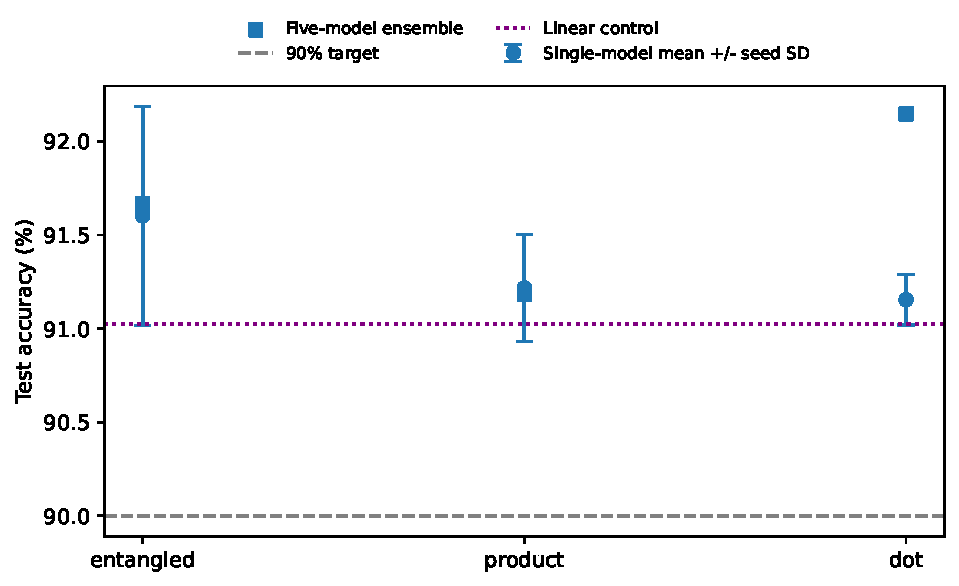
\includegraphics[width=\textwidth]{artifacts/native_quantum_accuracy/accuracy.pdf}
\caption{Retained comparison figure: single-model mean and standard deviation, ensemble outcomes, and classical linear control.}
\end{figure}

\section{Paired seed statistics}
Seeds are paired across kernels. Entangled minus product mean accuracy is $+0.38462$ percentage points, and entangled minus dot is $+0.44872$ points. These single-model means do not imply that their ensembles follow the same ordering.

The retained analysis performs exact sign-flip comparisons of paired seed differences, bootstraps seed means, and applies Holm correction to four comparisons: accuracy and AUROC against each of two controls. All four Holm-adjusted $p$ values are 1.0. With only five seeds, the smallest nonzero two-sided exact sign-flip $p$ is 0.0625. The bootstrap intervals characterize seed variation on this fixed cohort, not generalization to new patients.

\begin{table}[htbp]\centering\small
\begin{tabular}{llrr}\toprule
Contrast & Metric & Mean effect & Bootstrap 95\% interval\\\midrule
Entangled -- product & Accuracy, points & $+0.38462$ & $[-0.16026,+0.92949]$\\
Entangled -- dot & Accuracy, points & $+0.44872$ & $[0.00000,+0.89744]$\\
Entangled -- product & AUROC & $-0.00049$ & $[-0.00353,+0.00192]$\\
Entangled -- dot & AUROC & $+0.00058$ & $[-0.00185,+0.00333]$\\\bottomrule
\end{tabular}
\caption{Exploratory paired-seed effects. All associated Holm-adjusted $p$ values equal 1.0.}
\end{table}

\section{Paired ensemble comparisons}
McNemar's test focuses on images for which two classifiers disagree in correctness. The entangled--dot ensemble comparison has discordant counts 7 and 4 and exact two-sided $p=0.548828$. Entangled--product has discordant counts 2 and 5 and $p=0.453125$. Entangled--linear has counts 5 and 9 and $p=0.42395$. The direction of each count should be read from the saved analysis rather than inferred from the count order. None establishes a quantum accuracy benefit.

The analysis also retains paired DeLong comparisons of AUROC. Such paired-example statistics use the shared labeled examples, whereas seed comparisons use training-seed differences. These are different uncertainty sources. Repeated inspection of the same test cohort limits confirmatory interpretation of both.

\chapter{Independent verification of the quantum path}
\section{What is checked}
The analyzer verifies the frozen source and configuration hashes, feature metadata, encoder weights, dataset checksum, sample IDs, and labels. It recomputes normalization from the original training feature bank. It then recomputes CNN features from every original validation and test image and compares them with the stored banks.

For all fifteen neural checkpoints, inference is rerun and saved logits, probabilities, and reported metrics are checked. The linear model's coefficient array is also used to reproduce its output. This establishes that the result files correspond to the retained models rather than merely being typed into a table.

\section{Complete PennyLane inference}
Each of the ten quantum checkpoints replaces its training statevector-overlap backend with an independent PennyLane \code{default.qubit} compute--uncompute circuit. It evaluates every ordered token pair in each head and block for every test image. With $L=2$ blocks, $H=2$ heads, and $N=5$ tokens, there are
\begin{equation}
LHN^2=2\cdot2\cdot25=100
\end{equation}
circuit settings per image. This includes self-position pairs; query and key projections differ, so those entries cannot generally be assumed to have fidelity one.

Across 624 images and ten classifiers, the independently executed total is
\begin{equation}
624\cdot10\cdot100=624,000
\end{equation}
four-qubit settings, batched into 780 actual QNode calls. The verification records zero sampled shots because the simulator returns ideal probabilities. Zero shots means analytic simulator execution, not a probability estimate obtained without resource cost on hardware.

All argmax predictions match between the PyTorch gate implementation and PennyLane. The maximum observed logit disagreement is below $10^{-6}$, consistent with their differing numerical precision. The independently evaluated quantum ensembles reproduce the reported 91.67\% and 91.19\% accuracies.

\section{Tests and provenance}
The recorded complete suite has 24 passing tests. Relevant checks compare gate-prepared states with PennyLane, compare probabilities, perform numerical gradient checks, verify that suitable entangled outputs are nonseparable, check exact parameter matching, verify whole-model backend agreement, enforce training-only normalization, and check stochastic training resumption. Other tests cover earlier project components and remain included to preserve dependency coverage.

This does not prove behavior under decoherence, gate errors, readout errors, finite-shot attention noise, hardware connectivity constraints, or an independent clinical population. Those conditions were not part of the new accuracy execution.

\chapter{Earlier attempts and why they remain relevant}
\section{The older 88.94\% reference}
The earlier small-model ensemble with target-prior adjustment reached 88.9423\% for both fidelity and dot attention. Its target adaptation used unlabeled prediction information; labels were reserved for scoring. Earlier illustrative calculations that optimized a threshold using test labels or supplied the known positive count are not deployable methods and are excluded from the valid accuracy claim.

The new model does not use that target adaptation. It uses canonical test images, validation-calibrated probabilities, equal ensemble weights, and argmax. Consequently, the 2.72-point increase is a comparison of different complete pipelines, not an isolated optimizer or quantum-kernel ablation.

\section{Other unsuccessful branches}
\begin{table}[htbp]\centering\small
\begin{tabular}{p{7.4cm}r}\toprule
Branch & Relevant ensemble accuracy\\\midrule
Original small ensemble with valid prior adjustment & 88.94\%\\
Robust small model, entangled quantum attention & 89.10\%\\
Robust small model, product quantum attention & 89.74\%\\
Pretrained ResNet with enlarged 28-pixel source, entangled & 86.70\%\\
Pretrained ResNet with enlarged 28-pixel source, product & 86.70\%\\
Native-224 pretrained encoder, entangled & 91.67\%\\
Native-224 pretrained encoder, product & 91.19\%\\\bottomrule
\end{tabular}
\caption{Selected earlier outcomes and the final resolution branch. These are separate regimes rather than a single controlled treatment comparison.}
\end{table}

The robust small-backbone study piloted AdamW and sharpness-aware minimization (SAM). SAM perturbs parameters in the gradient direction, evaluates a second loss at the perturbed parameters, then updates the restored parameters. The shared pilot's average class-balanced validation NLL favored AdamW (approximately 0.19343 versus 0.22820 for SAM). SAM was not used in the final native branch. A longer-training branch and a trained convolutional-token branch also failed to establish a meaningful quantum advantage.

The separate bias-aware shot-allocation project studied measurement-error correction and sampling policy, rather than this ideal native classifier. Its joint correction/allocation primary MSE was approximately 55.1\% worse than the combined raw reference. That negative result remains documented. Neither its finite-shot measurements nor its accuracy can be substituted for measurements of the updated pretrained architecture.

\section{What is plausible, and what is measured}
Higher-resolution images plausibly expose useful detail and pretrained CNN representations plausibly reduce the burden on a small downstream head. The native and enlarged-28 outcomes are consistent with this explanation. However, the current results do not decompose the gain into separately randomized contributions from resolution, pretraining, optimizer, MixUp, EMA, and attention. A factorial or carefully planned ablation study would be needed for causal attribution.

\chapter{Reproduction and the UPDATED package}
\section{Directory map}
\begingroup\small
\begin{longtable}{p{6.8cm}p{7.2cm}}\toprule
Path & Purpose\\\midrule\endhead
\code{research/} & Byte-preserved source and supporting modules, including earlier algorithms required by imports and tests.\\
\code{configs/} & Original manifests and frozen hash locks; native manifest defines the completed study.\\
\code{runs/native_quantum_accuracy/} & Fifteen trained heads, linear coefficients, configurations, histories, predictions, and resumable checkpoints.\\
\code{artifacts/native_quantum_features/} & Frozen raw feature banks, training-only normalization, provenance metadata, and alignment audit.\\
\code{artifacts/native_quantum_accuracy/} & Summary, per-seed CSV, full verification, independent circuit predictions, ensembles, and plots.\\
\code{pretrained_models/} & Verified public ResNet-18 ImageNet weights.\\
\code{data/} & Small reference archive and local native-224 archive.\\
\code{tests/}, \code{verification/} & Executable tests, recorded logs, claims and known-failure documentation.\\
\code{environment/} & Recorded environment and full dependency lock.\\
\code{fetch_assets.py} & Restore the public raw archive after cloning and verify the encoder weights.\\
\code{verify_package.py} & Check packaged file bytes against the SHA256 inventory.\\
\code{PACKAGE_CONTENTS.json} & Relative paths, file sizes, and exact SHA256 records.\\\bottomrule
\end{longtable}
\endgroup

\section{Running the retained study}
All commands assume the current directory is \code{UPDATED}, because the original experiment uses relative paths. The recorded environment was Python 3.14.2, PyTorch 2.14 CPU, torchvision 0.29, and PennyLane 0.45.1, with no available GPU or QPU. The environment lock records the actual installed packages; a new clean installation has not independently been validated merely by writing this report.
\begin{lstlisting}[language={},caption={Reproduce from the standalone folder.}]
cd UPDATED
python -m pip install -r requirements.txt
python fetch_assets.py
python verify_package.py
python tests/run_suite.py
python -m research.quantum_native_accuracy analyze
\end{lstlisting}
The analysis recomputes every validation/test feature and every quantum test overlap, so it is more expensive than loading a saved summary. On a CPU it can take several minutes. The native adapter automatically requests full circuit verification.

\section{Preparing or training a new study}
The executable exposes \code{prepare}, \code{freeze}, \code{run}, and \code{analyze}. Prepare builds feature banks; freeze records source, manifest, weight, and feature hashes; run trains or resumes conditions; analyze verifies and reports them. The completed package is already prepared, frozen, and trained. Running \code{run} reuses completed results instead of silently retraining them.

To conduct a fresh experiment, create a separate copy with a distinct experiment namespace and new provenance. Do not edit the frozen computational files in this package or refreeze them after looking at these test outcomes. Regenerating caches with a different software stack may produce numerically close but byte-different files; such changes do not satisfy the old cache hash lock and should form a new experiment rather than replacing historical evidence.

\section{GitHub distribution and asset handling}
The local package includes the official 214 MB native archive. It exceeds the normal GitHub per-file limit, so that archive is ignored in ordinary Git and restored through the included fixed-URL, checksum-verified downloader. Its size and SHA256 are still recorded in the package inventory. The smaller reference archive, encoder weights, feature caches, checkpoints, predictions, and report are distributed with the source.

The copying process preserves original source bytes so the existing freeze remains meaningful after relocation. The earlier root documents, dashboard, presentation, and experiments are not overwritten. A copy of the legacy dashboard and one original small-model checkpoint is included only for its existing integration tests; it does not serve the new native classifier. This package's report describes the updated architecture; the original presentation remains a record of the earlier study.

\chapter{Contribution, limitations, and defensible presentation}
\section{A precise contribution statement}
The project implements and verifies a complete hybrid image classifier in which a frozen pretrained encoder feeds a compact transformer using four-qubit entangled state-fidelity attention. It evaluates that classifier alongside a product-state circuit, a parameter-matched dot-attention head, and a simple linear classifier under a shared protocol. It retains failed attempts and independently checks complete circuit inference. These are concrete engineering and experimental contributions.

A defensible presentation statement is:
\begin{quote}
We built a hybrid classifier using pretrained image features and four-qubit quantum fidelity attention. Its entangled five-model ensemble achieved 91.67\% on all 624 official test images, and independent PennyLane inference reproduced those decisions. The gain over our earlier model accompanies higher-resolution data and external pretraining; our matched classical ensemble reached 92.15\%, so we do not claim quantum superiority.
\end{quote}

\section{Publication and novelty}
Transfer learning, angle encoding, repeated data encoding, entangling circuits, and fidelity-based comparison have prior art. Their combination with an accuracy number does not automatically constitute a new publishable algorithm. This report does not claim the four-qubit circuit is an invention absent from the literature. The retained novelty-gate documents record the prior-art checks performed before the new implementation.

Possible stronger research directions include a genuinely isolating entanglement ablation, prospectively fixed testing on another cohort, calibrated finite-shot resource comparisons, or a method addressing a demonstrated limitation with a clearly distinguished mathematical contribution. These are future possibilities, not completed results. More tuning on the already inspected test split would not provide independent evidence.

\section{Remaining limitations}
\begin{itemize}
\item Results use an already inspected official cohort, not independent external confirmation.
\item Higher resolution and ImageNet pretraining confound attribution of improvement over the old regime.
\item The best matched classical ensemble is more accurate; no statistically established quantum advantage appears.
\item Product versus entangled removes two circuit components, preventing attribution solely to entanglement.
\item Four-qubit ideal simulation says nothing by itself about noisy or finite-shot hardware accuracy.
\item Five seeds give limited statistical resolution. Seeds are not independent patient populations.
\item Dataset ordering checks do not prove absence of patient overlap or clinical deployment validity.
\item The native classifier's measured quantum resources exclude hardware execution, transpilation, and shots; frozen CNN costs also remain classical costs.
\end{itemize}

\appendix
\chapter{Implementation source used for the result}
The following files are the retained implementation, not illustrative pseudocode. Auxiliary modules and exact configurations are supplied in the package. The robust module also contains the older augmentation and SAM utilities; those routines are not activated by the native transfer trainer. The native adapter changes runtime namespaces and loading resolution without changing the preceding frozen computational files.
\section{Quantum gates and attention}
\lstinputlisting[language=Python]{research/quantum_robust.py}
\section{Pretrained encoder and transfer head}
\lstinputlisting[language=Python]{research/quantum_transfer.py}
\section{Training, selection, and linear control}
\lstinputlisting[language=Python]{research/quantum_transfer_experiment.py}
\section{Native-resolution adapter and correspondence checks}
\lstinputlisting[language=Python]{research/quantum_native_accuracy.py}
\section{Frozen experiment configuration}
\lstinputlisting[language={}]{configs/native_quantum_accuracy.json}

\begin{thebibliography}{9}
\bibitem{medmnist} MedMNIST team. MedMNIST+: standardized biomedical classification datasets with multiple size options. Official dataset release, Zenodo record 10519652. \url{https://zenodo.org/records/10519652}. Accessed 2 October 2026.
\bibitem{resnetdocs} PyTorch torchvision. ResNet-18 model and ImageNet weight preprocessing documentation. \url{https://docs.pytorch.org/vision/stable/models/generated/torchvision.models.resnet18.html}. Accessed 2 October 2026.
\bibitem{mari} A. Mari, T. R. Bromley, J. Izaac, M. Schuld, and N. Killoran. Transfer learning in hybrid classical--quantum neural networks. \emph{Quantum} 4, 340 (2020). \url{https://arxiv.org/abs/1912.08278}.
\bibitem{reupload} A. P\'erez-Salinas, A. Cervera-Lierta, E. Gil-Fuster, and J. I. Latorre. Data re-uploading for a universal quantum classifier. \emph{Quantum} 4, 226 (2020). \url{https://arxiv.org/abs/1907.02085}.
\end{thebibliography}
\end{document}
